%%%%%%%%%%%%%%%%%%%%%%%%%%%%%%%%%%%%%%%%%%%%%%%%%%%%%%%%%%%%%%%%%%%%%%%%%%%%%%%%
% reconstruction.tex:
%%%%%%%%%%%%%%%%%%%%%%%%%%%%%%%%%%%%%%%%%%%%%%%%%%%%%%%%%%%%%%%%%%%%%%%%%%%%%%%%
\chapter{Event Reconstruction}
\label{sec:reco_chapter}
%%%%%%%%%%%%%%%%%%%%%%%%%%%%%%%%%%%%%%%%%%%%%%%%%%%%%%%%%%%%%%%%%%%%%%%%%%%%%%%%

Electrons, muons and jets expected from \WR and \nul decays traverse multiple CMS sub-detectors, as shown in 
Figure \ref{fig:particleTrajectories}.  Their trajectories and energies were measured from charged particle tracks 
reconstructed by the silicon tracker and muon detectors, and energy deposits reconstructed by the calorimeters.  The 
high energy of expected leptons and jets motivated the use of specific lepton and jet reconstruction algorithms 
described here.  These algorithms combine measurements from multiple CMS sub-detectors to measure the trajectory 
and energy of each particle with the best resolution.  For charged particles, initial energy and trajectory 
measurements are made using tracks reconstructed from signals measured in the silicon tracker.

\begin{figure}[h]
	\centering
	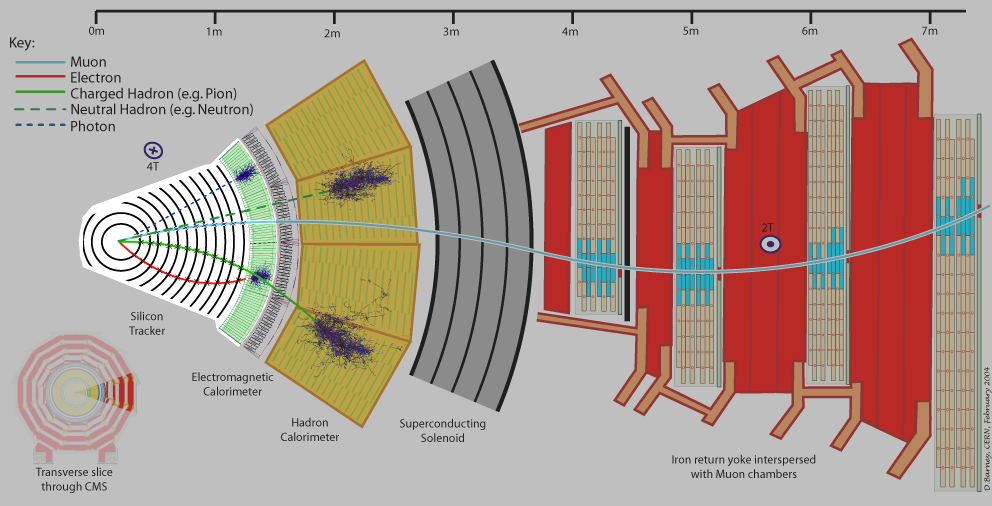
\includegraphics[width=0.75\textwidth]{figures/flowOfParticlesThroughCMS.png}
	\caption{Typical trajectories of particles travelling through CMS, from CERN.}
	\label{fig:particleTrajectories}
\end{figure}


\section{Track Reconstruction}
\label{sec:trkReco}
Charged particles are reconstructed as helical tracks from signals in the silicon tracker.  An interative algorithm 
reconstructs tracks from the highest energy signals and signals closest to the IP, and progressively includes outer layer 
signals using a Kalman filter to link signals in successive layers.  Signals in succesive layers are linked only if they 
pass a $\chi^{2} =$ 30 threshold \cite{trackerPerformanceInCollisions}, and during linking it is assumed that particles do 
not lose more than a few percent of their initial energy when traversing the entire tracker.  Upon reaching the outermost 
tracker layer, the collection of signals linked into continuous helical tracks are removed from the list of track candidates, 
and the algorithm restarts using signals in the innermost pixel layers that have lower energy or are further from the IP.  Isolated muons 
were used to estimate the tracker reconstruction efficiency; and those with $\pt > 0.9$ $\GeV$ and $|\eta| < 2.4$ 
were reconstructed with essentially 100\% efficiency \cite{trackerPerformanceInCollisions}.  After reconstructing all 
tracks, each point where two or more tracks originated is identified as an interaction vertex, and its position relative 
to the IP is measured.  Again muons were used to estimate the tracker vertex resolution; for muons reconstructed with 
$|\eta| < 1.4$, $\pt = 100$ $\GeV$ and associated with a vertex, the vertex position relative to the IP was measured 
with 10 and 30 $\mu$m resolutions in the transverse (r-$\phi$) and longitudinal ($z$) directions.

Tracks from muons and charged hadrons are reconstructed as described previously, but a second track reconstruction 
algorithm was used to reconstruct electron tracks.  The silicon tracker contains, depending on $\eta$, 1 to 2 radiation 
lengths of material, and $\sim$35\% of electrons that traverse the tracker lose more than 70\% of their initial energies 
through bremsstrahlung \cite{trackerPerformanceInCollisions}.  The electron track reconstruction algorithm differs from 
the muon and charged hadron track algorithm in that it models the electron energy loss in successive silicon layers 
as a sum of multiple Gaussians, and requires that signals in successive layers have $\chi^{2} =$ 2000 or better before a 
link is made.  Electrons traversing the tracker lose energy that cannot be measured by the tracker, but, by using a 
dedicated electron track reconstruction algorithm, electrons with $\pt > 20$ $\GeV$ and $|\eta| < 2.5$ are reconstructed 
in the tracker with an efficiency of 97\% or better \cite{gsfPerformanceInCollisions}.


\section{Energy Reconstruction}
\label{sec:enrgReco}
The total energies of photons and electrons, and partial energies of hadrons produced by pp interactions are measured 
in the ECAL.  Photons, electrons, and hadrons impinging on the ECAL generate signals in the ECAL crystals that are 
converted into $\Et$ measurements.  The upstream tracker material causes $\sim$35\% .


%After traversing the tracker, electrons impinged on ECAL crystals and showered into lower energy $e^{\pm}$s, and 
%electron energies were measured through these showers.  Approximately 94\% of an electron's energy coming 
%into the ECAL was deposited over a 3 $\times$ 3 crystal area, but due to bremsstrahlung in the tracker an electron's 
%total energy was usually deposited over a larger area.  To measure the total energy of each electron, ECAL energy deposits 
%were reconstructed in superclusters (SCs) centered on the most energetic crystal, and were 3 or more crystals wide 
%in $\eta$ depending on the electron shower shape.  SCs were 5 or more crystals wide in $\phi$, as shown in Figure 
%\ref{fig:eleTrackAndSC}, to measure the energy lost by electrons through bremsstrahlung in the tracker.  Once a SC 
%was reconstructed its $(\eta, \phi)$ position was calculated as the energy-weighted average position of all crystals 
%in the SC, and this position was compared to $(\eta, \phi)$ trajectories of electron candidate tracks to identify 
%an electron.  Each reconstructed electron was identified as a SC that geometrically matched at least one candidate 
%track to within 1.1$^{\circ}$, about 6 crystals wide, in $\phi$, and within 0.004 units, less than $\frac{1}{2}$ a 
%crystal wide, in $\eta$.  The ECAL was used to determine reconstructed electron energies and positions.  The energy 
%resolution for electrons from $Z \rightarrow ee$ decays with $\Et \approx 45$ $\GeV$ was better than 2\% for 
%$|\eta| < 0.8$, and was between 2\% and 5\% elsewhere \cite{ecalPerformanceInCollisions}.  The position resolution 
%for single electrons from $W \rightarrow e\nu$ decays in the barrel (endcap) was 0.17$^{\circ}$ (0.29$^{\circ}$) in 
%$\phi$, and 0.001 (0.002) units in $\eta$.

%Through hadronization, photon radiation, and leptonic weak decays, quarks produced jets of photons, hadrons, and leptons.  
%Thus, photons, electrons and muons, and charged and neutral hadrons were reconstructed before jets were built.  Photons 
%were reconstructed in the ECAL as superclusters that did not overlap in $(\eta,\phi)$ with any energy deposits measured 
%in the HCAL, and were separated from any reconstructed track by at least 1.1$^{\circ}$ in $\phi$ and 1 ECAL crystal in $\eta$.  
%Charged and neutral hadrons were reconstructed in the HCAL as individual or multiple neighboring towers, and were 
%reconstructed in the ECAL as superclusters that overlapped with the HCAL towers \cite{pflowJetRecoInCollisions}.  Each 
%charged hadron was identified as a track, reconstructed as described for muons in Section \ref{sec:muReco}, that extrapolated 
%to the $(\eta,\phi)$ area of the ECAL SC or at least one of the HCAL towers.  Each neutral hadron was identified as an HCAL 
%energy cluster, and possibly an ECAL SC, that did not overlap with any reconstructed track in $(\eta,\phi)$.  After 
%individual particles were reconstructed, jets were built from clusters of individual particles, as shown in Figure 
%\ref{fig:jetClustering}.


%RESUME HERE


\section{Muon Reconstruction}
\label{sec:muReco}
%from \cite{trackerPerformanceInCollisions}
%muons with $|\eta| < 1.4$ and $\pt = 100$ $\GeV$ were measured with a $\pt$ resolution of $\sim$2.8\%.

Muons were first reconstructed as tracks from signals in the silicon tracker.  An interative algorithm started 
by reconstructing tracks from the highest energy signals and signals closest to the IP, and progressed to outer layers 
using a Kalman filter to link signals between successive layers.  Once the algorithm reached the outermost tracker 
layer the signals associated with tracks were removed from the list of track candidates, and a new iteration of track 
reconstruction started with signals in the innermost pixel layers that had lower energy or were further 
from the IP.  It was assumed that the magnetic field was uniform, so tracks were reconstructed as perfect helixes 
from signals in consecutive layers.  If two or more tracks shared a common origin point, that point was reconstructed 
as an interaction vertex, whose position was measured relative to the IP.  Isolated muons with 
$\pt > 0.9$ $\GeV$ and $|\eta| < 2.4$ were reconstructed with essentially 100\% efficiency \cite{trackerPerformanceInCollisions}.  
Muons with $|\eta| < 1.4$ and $\pt = 100$ $\GeV$ and their vertices were measured with resolutions of approximately 
2.8\% in $\pt$, and 10 and 30 $\mu$m in transverse and longitudinal distances from the IP.  Muon trajectories and 
initial energies were determined by tracker measurements, and their energies were refined by muon detector measurements.

After traversing the calorimeters and the magnet, muons were reconstructed as tracks from signals in muon detector chambers.  
First, local reconstruction was run to build track segments in individual chambers, then an iterative track 
reconstruction algorithm built continuous tracks from multiple segments.  The muon track reconstruction algorithm started 
with track segments in the inner muon chambers, then iterated outward and built longer tracks across multiple chambers 
using a Kalman filter.  The algorithm estimated the effects of energy losses, inhomogenous magnetic fields, and multiple 
scattering when linking segments between chambers, and updated all track parameters after including measurements 
from each new chamber.  Once the algorithm incorporated measurements from the outermost chambers, a Kalman filter 
was applied to the reconstructed tracks, starting with the outermost chamber segments and working towards the 
innermost chamber segments, to ensure the tracks were built in a self-consistent way \cite{muonRecoFirstCollisions}.  

Muons were reconstructed and their momenta were determined using silicon tracker and muon detector measurements.  
Tracks reconstructed in the muon detectors were extrapolated back to the outermost silicon tracker layer, and in the 
plane of the silicon strip each reconstructed muon was identified as a muon detector track that matched a silicon 
tracker track to within 3 cm.  After reconstruction, the $\pt$ of each muon was calculated using the following procedure.  
Four muon reconstruction algorithms fitted four continuous tracks \cite{cmsMuonRecoRunTwo} to silicon tracker and muon 
detector signals to estimate a muon's trajectory through CMS, as represented in Figure \ref{fig:particleTrajectories}.  Each 
algorithm combined muon detector and silicon tracker measurements in a different way, and could exclude measurements with 
large uncertainty.  The quality of each continuous track was identified by a fit uncertainty $\chi^{2}/nDOF$ and momentum 
uncertainty $\sigma(\pt)/\pt$.  The track with the lowest $\chi^{2}/nDOF$ and momentum uncertainty $\sigma(\pt)/\pt < 0.3$ was 
used to calculate the reconstructed muon momentum.  For muons with $\pt \lesssim 100$ $\GeV$ this procedure used tracker 
measurements almost exclusively to determine the muon momentum; as stated earlier, muons with $|\eta| < 1.4$ and $\pt = 100$ 
$\GeV$ were measured with a $\pt$ resolution of approximately 2.8\%.  As the muon $\pt$ increased above 100 $\GeV$ the 
silicon tracker $\pt$ resolution degraded faster than the muon detector $\pt$ resolution, and it became advantageous to 
combine measurements from both detectors.  Muons with $\pt > 200$ $\GeV$ were expected in a significant fraction of 
$\WR \rightarrow \mu\mu jj$ events (Table \ref{tab:wrHighPtMuons}), and for $|\eta| < 0.9$ and $200 < \pt < 400$ $\GeV$ 
they were measured with a $\pt$ resolution of 3.2\%; for $\pt > 400$ $\GeV$ the resolution was better than 6\% \cite{cmsMuonRecoRunTwo}.

\begin{table}[h]
	\caption{Fraction of expected $\WR \rightarrow \mu\mu jj$ events that had at least one muon with $\pt > 200$ $\GeV$. 
	($\mnul = \frac{1}{2}\mWR$)}
	\label{tab:wrHighPtMuons}
	\centering
	\begin{tabular}{c|c}
		\mWR ($\TeV$) & Fraction of events with at least one high-$\pt$ muon (\%) \\  \hline
		1.0 &  80.  \\
		2.0 &  95.  \\ 
		3.0 &  98.  \\ \hline
	\end{tabular}
\end{table}

Muons reconstructed in $Z \rightarrow \mu\mu$ events were used to match the muon energy scale and resolution in data 
and simulations used to estimate the \WR signal and ST backgrounds.  The di-muon mass ($M_{\mu\mu}$) distribution in 
$Z \rightarrow \mu\mu$ events was compared between data and simulations, and two differences were found.  In simulations 
the $M_{\mu\mu}$ peak position was higher in energy, indicating a higher muon energy scale, and the $M_{\mu\mu}$ distribution width 
was smaller, indicating a better muon energy resolution than what was stated previously.  These differences 
were resolved by increasing the momenta of muons reconstructed in data by a small fixed percentage, and smearing the momenta 
of muons reconstructed in all simulations by a small positive value multiplied by a Gaussian random number that changed 
with every event.


\section{Electron Reconstruction}
\label{sec:eleReco}
Electrons ($e^{\pm}$) were the only particles from \WR decays expected to lose more than a few percent of their 
energy before reaching the ECAL.  One to two radiation lengths of material, depending on $\eta$, was in front of 
the ECAL \cite{ecalPerformanceInCollisions}, and about 35\% of electrons lose more than 70\% of their initial energy 
through bremsstrahlung before reaching the ECAL \cite{trackerPerformanceInCollisions}.  The curvature of electrons 
in the magnetic field meant that bremsstrahlung photons emitted by the electrons, in general, struck the ECAL 
at $\eta$ values similar to that of the electron, but at different $\phi$ coordinates.  The tracker could not detect 
these photons, but knowledge of electron bremsstrahlung was incorporated into a dedicated electron track reconstruction 
algorithm.  The fractional energy lost by electrons traversing a tracker layer through bremsstrahlung was expected to 
have a distribution described by the Bethe-Heitler formula, and this energy loss was approximated as a sum of 
several Gaussians in the electron track reconstruction algorithm.  The electron algorithm was otherwise identical to 
the muon track reconstruction algorithm, except that the $\chi^{2}$ threshold used to 
associate tracker signals with a trajectory was loosened from 30 to 2000 \cite{trackerPerformanceInCollisions}.  This 
facilitated the reconstruction of electron tracks whose trajectories deviated from expectations due to bremsstrahlung.  
Bremsstrahlung increased the uncertainty of electron position and energy measurements made by the tracker relative to 
measurements made by the ECAL, so the kinematics of electrons expected from \WR decays was measured using the ECAL.

After traversing the tracker, electrons impinged on ECAL crystals and showered into lower energy $e^{\pm}$s, and 
electron energies were measured through these showers.  Approximately 94\% of an electron's energy coming 
into the ECAL was deposited over a 3 $\times$ 3 crystal area, but due to bremsstrahlung in the tracker an electron's 
total energy was usually deposited over a larger area.  To measure the total energy of each electron, ECAL energy deposits 
were reconstructed in superclusters (SCs) centered on the most energetic crystal, and were 3 or more crystals wide 
in $\eta$ depending on the electron shower shape.  SCs were 5 or more crystals wide in $\phi$, as shown in Figure 
\ref{fig:eleTrackAndSC}, to measure the energy lost by electrons through bremsstrahlung in the tracker.  Once a SC 
was reconstructed its $(\eta, \phi)$ position was calculated as the energy-weighted average position of all crystals 
in the SC, and this position was compared to $(\eta, \phi)$ trajectories of electron candidate tracks to identify 
an electron.  Each reconstructed electron was identified as a SC that geometrically matched at least one candidate 
track to within 1.1$^{\circ}$, about 6 crystals wide, in $\phi$, and within 0.004 units, less than $\frac{1}{2}$ a 
crystal wide, in $\eta$.  The ECAL was used to determine reconstructed electron energies and positions.  The energy 
resolution for electrons from $Z \rightarrow ee$ decays with $\Et \approx 45$ $\GeV$ was better than 2\% for 
$|\eta| < 0.8$, and was between 2\% and 5\% elsewhere \cite{ecalPerformanceInCollisions}.  The position resolution 
for single electrons from $W \rightarrow e\nu$ decays in the barrel (endcap) was 0.17$^{\circ}$ (0.29$^{\circ}$) in 
$\phi$, and 0.001 (0.002) units in $\eta$.

\begin{figure}[h]
	\centering
	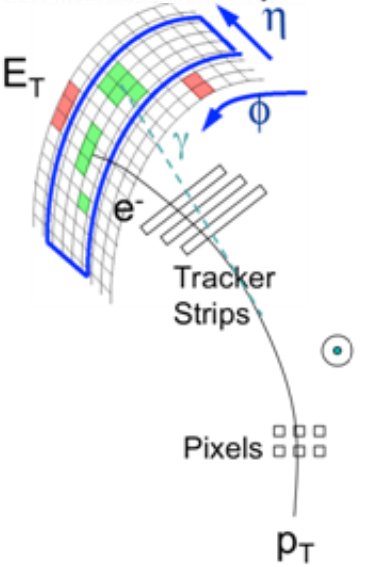
\includegraphics[width=0.75\textwidth]{figures/electronTrackAndSupercluster.png}
	\caption{The trajectory of a typical electron through the tracker and the ECAL.}
	\label{fig:eleTrackAndSC}
\end{figure}

Electrons reconstructed in $Z \rightarrow ee$ events were used to match the electron energy scale and resolution in data 
and simulations used to estimate the \WR signal and ST backgrounds.  The di-electron mass ($M_{ee}$) distribution in 
$Z \rightarrow ee$ events was compared between data and simulations, and two differences were found.  In simulations 
the $M_{ee}$ peak position was higher in energy, indicating a higher electron energy scale, and the $M_{ee}$ distribution width 
was smaller, indicating a better electron energy resolution than what was stated previously.  These differences 
were resolved by increasing the energies of electrons reconstructed in data by a small fixed percentage, and smearing the energies 
of electrons reconstructed in all simulations by a small positive value multiplied by a Gaussian random number that changed 
with every event.


\section{Jet Reconstruction}
\label{sec:jetReco}
Through hadronization, photon radiation, and leptonic weak decays, quarks produced jets of photons, hadrons, and leptons.  
Thus, photons, electrons and muons, and charged and neutral hadrons were reconstructed before jets were built.  Photons 
were reconstructed in the ECAL as superclusters that did not overlap in $(\eta,\phi)$ with any energy deposits measured 
in the HCAL, and were separated from any reconstructed track by at least 1.1$^{\circ}$ in $\phi$ and 1 ECAL crystal in $\eta$.  
Charged and neutral hadrons were reconstructed in the HCAL as individual or multiple neighboring towers, and were 
reconstructed in the ECAL as superclusters that overlapped with the HCAL towers \cite{pflowJetRecoInCollisions}.  Each 
charged hadron was identified as a track, reconstructed as described for muons in Section \ref{sec:muReco}, that extrapolated 
to the $(\eta,\phi)$ area of the ECAL SC or at least one of the HCAL towers.  Each neutral hadron was identified as an HCAL 
energy cluster, and possibly an ECAL SC, that did not overlap with any reconstructed track in $(\eta,\phi)$.  After 
individual particles were reconstructed, jets were built from clusters of individual particles, as shown in Figure 
\ref{fig:jetClustering}.

\begin{figure}[h]
	\centering
	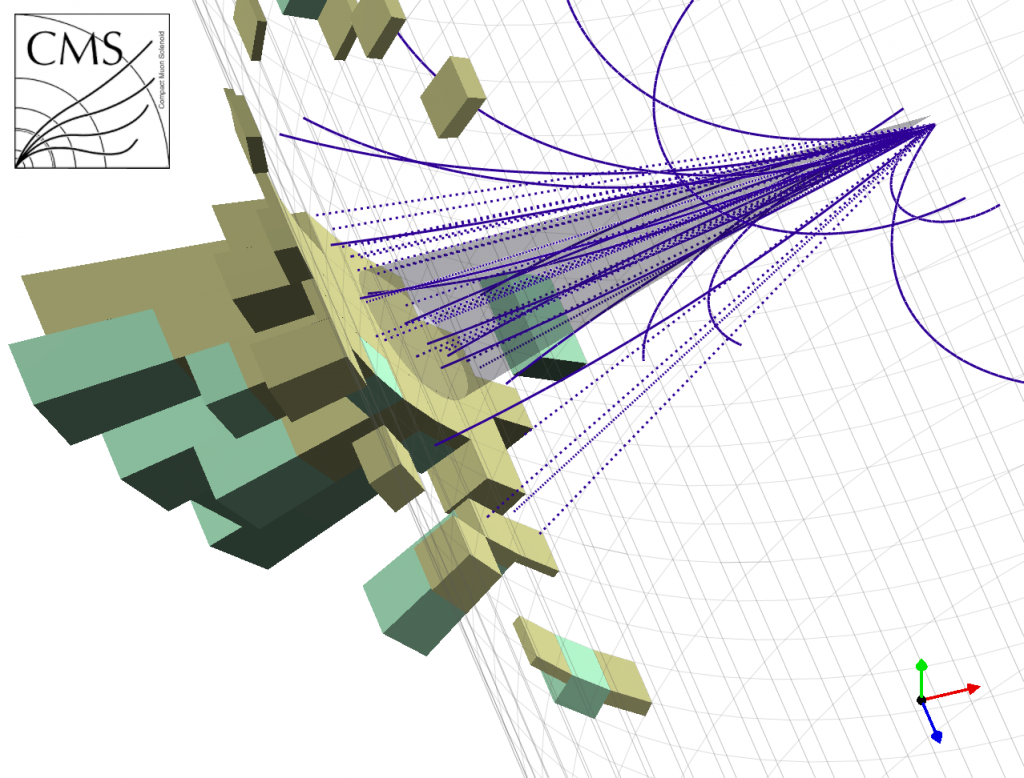
\includegraphics[width=0.75\textwidth]{figures/jetClusteringInCMS.png}
	\caption{A cone of reconstructed particles clustered into a jet, with the reconstructed vertex on the right.  
	From the CMS Experiment.}
	\label{fig:jetClustering}
\end{figure}

The high instantaneous luminosity of pp collisions delivered by the LHC almost always resulted in collision events with 
multiple reconstructed vertices, which represented pileup interactions.  The dominant effect of pileup interactions was 
the production of additional quarks and gluons, and thus additional jets.  Pileup jets originating from charged hadrons 
were significantly reduced by excluding charged hadrons from jet reconstruction that were not associated with the vertex, 
the primary vertex, that had the highest $\sum \pt$ in the event.  Neutral hadrons produced by pileup interactions contributed 
to the energies of all reconstructed jets, in addition to creating new jets.  Their effect was reduced by measuring the average 
neutral hadron energy density, $\rho$, over all $(\eta,\phi)$ in each event, and reducing the energy of jets reconstructed in each 
event by $\rho$ multiplied by each jet's area \cite{pileup1,pileup2}.

In each collision event, every reconstructed particle was considered a jet candidate except the charged hadrons from pileup 
vertices.  Candidate particles were clustered into jets using the anti-$k_{T}$ algorithm \cite{antikt} to cluster particles 
based on their $\pt$ and distance $\Delta R$ from the jet axis.  The jet axis was defined initially by a charged hadron, and 
was updated iteratively based on the $\pt$ weighted $(\eta,\phi)$ trajectories of all jet constituents.  Jets were built 
from particles reconstructed anywhere in the detector, but the anti-$k_{T}$ algorithm used a cone size of $\Delta R = 0.4$ to reduce the 
likelihood of having a jet constituent that was $\Delta R > 0.4$ away from the jet axis.  Once a jet was clustered its 
energy was determined as the $\sum \pt$ of all jet constituents.  Reconstructing jets from individual particles benefitted 
from the energy resolution of the tracker and the ECAL, and as a result jets with $\pt > 50$ $\GeV$ and $|\eta| < 3.0$ were 
measured with $\pt$ resolution better than 15\% \cite{jetResolutionInCollisions}.

The energies of reconstructed jets were corrected based on several observed effects.  As described previously, neutral 
hadrons produced in pileup interactions contributed to the energies of all jets, and their contributions were mitigated by 
reducing each jet's energy based on its $(\eta,\phi)$ area.  Following this subtraction, jets reconstructed in dijet, $Z$+jet, 
or $\gamma$+jet events were used to match the jet energy scale and resolution in data and simulations used to estimate the 
signal and backgrounds.  In simulated events jets were found to have a different energy scale and resolution, and these 
differences were resolved by correcting jet energies in data and simulated events, using methods described elsewhere \cite{jetpaper}.  


\section{Conclusion}
\label{sec:recoConclusion}
Energetic electrons, muons and jets produced in collisions were reconstructed using several CMS sub-detectors and high energy 
reconstruction algorithms.  Additional selections were applied to reconstructed leptons and jets to increase sensitivity to the \WR 
signal relative to ST backgrounds that produced $\ell\ell jj$ events.

%%%%%%%%%%%%%%%%%%%%%%%%%%%%%%%%%%%%%%%%%%%%%%%%%%%%%%%%%%%%%%%%%%%%%%%%%%%%%%%%
